\chapter{Dart}

\section{Introduzione al linguaggio}
\textbf{Dart} è un linguaggio di programmazione ottimizzato per applicazioni multipiattaforma sviluppato da Google. Questo linguaggio è nato nel 2011 per lo sviluppo di applicazioni Web. Lo scopo di Dart è quello di risolvere i problemi strutturali di \textit{JavaScript} che non possono essere risolti con l'evoluzione del linguaggio stesso. Queste affermazioni sono state scritte in una mail interna di Google, in qui viene definito \textit{Dash} (il nome provvisorio di Dart quando il progetto era ancora in una fase embrionale) il linguaggio che dovrà \textit{"sostituire JavaScript come lingua franca per lo sviluppo web sulla piattaforma web aperto"}\cite{mail_google}.

Dart offre delle prestazioni migliori, rende lo sviluppo più semplice e introduce migliori funzionalità legate alla sicurezza. Nonostante nei primi anni questo linguaggio non riuscì a riscuotere il successo che il team di Google sperava, l'azienda decise di utilizzarlo per lo sviluppo di applicazioni mobile \textbf{\textit{platform-independent}}, ovvero, per l'implementazione del framework \textit{Flutter}. Inoltre, tramite questo linguaggio è possibile creare applicazioni anche per \textit{desktop} (Windows, macOS, Linux/Unix-based e Fuchsia), lato \textit{server} e per dispositivi \textit{IoT}.

Gli obiettivi principali che il team di sviluppo di Google si è preposto di perseguire per la realizzazione di Dart, sono:
\begin{enumerate}
	\item \textbf{Portabilità}: creare un linguaggio strutturato e flessibile per lo sviluppo di applicazioni per il Web e la possibilità di sviluppare applicazioni per tutti i device sul Web.;
	\item \textbf{Produttività}: rendere Dart un linguaggio semplice e familiare ai programmatori, ovvero, con una \textit{curva di apprendimento} bassa. Inoltre deve avere una sintassi chiara e concisa;
	\item \textbf{Velocità}: i costrutti del linguaggio devono fornire delle alte performance ed un avvio veloce delle applicazioni;
\end{enumerate}

In questo capitolo si andranno ad approfondire gli aspetti fondanti del linguaggio e gli aspetti più rilevanti, necessari per la realizzazione del progetto, senza elencare tutte le singole caratteristiche e funzionalità \cite{tour_linguaggio}.

\section{Paradigmi}
Dart è un linguaggio \textit{multiparadigma}, ovvero, è un linguaggio principalmente \textit{orientato agli oggetti} ma offre anche le potenzialità della \textit{programmazione funzionale}, della \textit{programmazione imperativa} e della \textit{programmazione event-driven}. Analogamente al linguaggio Java, fa uso di un \textit{garbage collector}, ovvero, un meccanismo che libera la memoria occupata da oggetti che non sono più utilizzati dal programma. L'utilizzo di più paradigmi permette di ottenere un linguaggio flessibile e che unisce i vantaggi di ogni paradigma \cite{dart_paradigm}.

\subsection{Programmazione reattiva}
Oltre ai paradigmi già citati, Dart integra anche la \textit{programmazione reattiva}, fondamentale per la realizzazione di applicazioni per dispositivi mobile prestanti, veloci ed efficienti \cite{dart_paradigm}. 
Questo paradigma si fonda sulla nozione del cambiamento dei valori nel tempo, a seguito del verificarsi di un evento, e la conseguente propagazione di tali cambiamenti. Diverse fonti forniscono delle definizioni differenti:
\begin{enumerate}
	\item \textbf{Reactive Manifesto}: Reactive Systems are Responsive, Elastic, Resilient, Message Driven \cite{reactive_manifesto};
	\item \textbf{Wikipedia}: Reactive Programming is a programming paradigm oriented around data flows and the propagation of change \cite{reactive_programming_wikipedia}.
\end{enumerate}
Nonostante le differenze, si possono trarre dei concetti che vengono condivisi da entrambe le definizioni. In particolare, i concetti su cui si basa la programmazione reattiva, sono:
\begin{enumerate}
	\item La nozione di \textit{flusso di dati} e la \textit{propagazione} dei cambiamenti nell'applicazione;
	\item La possibilità di gestire facilmente dei \textit{flussi asincroni}, sia che essi siano di dati o di eventi;
	\item È un paradigma che ha una forte correlazione con la programmazione event-driven.
\end{enumerate}

\begin{figure}
	\begin{center}
		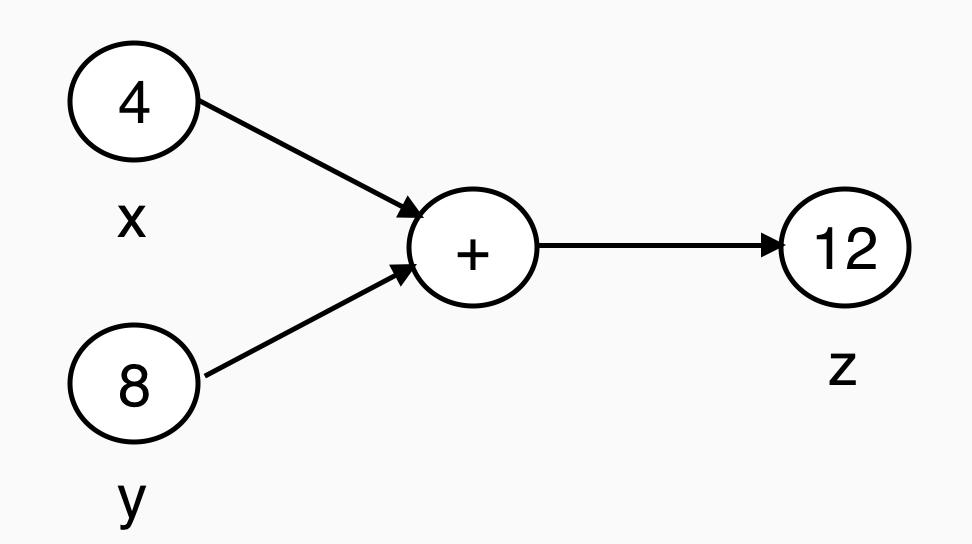
\includegraphics[scale=0.6]{dipendenza_programmazione_reattiva}
		\caption[Programmazione reattiva]{Rappresentazione della dipendenza delle variabili dell'esempio.}
		\label{figura:dipendenza_programmazione_reattiva}
	\end{center}
\end{figure}

Dal punto di vista dello sviluppo, questo paradigma offre un importante vantaggio, in quanto il programmatore deve focalizzare la sua attenzione sul \textit{che cosa deve fare} l'applicazione e può delegare la gestione al linguaggio su \textit{quando deve essere fatto}. In questo modo, al verificarsi di un evento, i cambiamenti vengono propagati attraverso la rete delle \textbf{dipendenze computazionali} dal sottostante modello di esecuzione. Per mostrare concretamente i vantaggi della programmazione reattiva, si procede con l'esposizione di un esempio:
\begin{center}
	\begin{lstlisting}
			x = 4;
			y = 8;
			z = x + y;
	\end{lstlisting}
\end{center}
La redazione di questo semplice codice con un linguaggio imperativo fa si che il risultato di \verb|z| sia 12 e che tale risultato non verrà modificato fino a quando non verrà assegnato esplicitamente un nuovo valore a tale variabile. In altri termini, \verb|z| rappresenterà sempre la somma dei due valori iniziali. L'assegnamento di nuovi valori alle variabili iniziali non influenzeranno il risultato contenuto in \verb|z|. L'esecuzione di questo codice, scritto con un linguaggio che supporta la programmazione reattiva, mantiene aggiornato il valore di \verb|z| ogni volta che almeno uno dei due addendi viene modificato: alla modifica di una delle due variabili, durante l'esecuzione del codice, viene automaticamente aggiornato il contenuto della variabile \verb|z|. Nel contesto della programmazione reattiva, la variabile \verb|z| è definita come \textit{dipendente} dalle variabili \verb|x| e \verb|y|. È possibile rappresentare graficamente la relazione di dipendenza tra le variabili del codice di esempio (Figura 4.1) \cite{reactive_programming_wikipedia}.

Il concetto di dipendenza viene realizzato attraverso l'implementazione di \textit{ascoltatori}, che riescono ad intercettare i cambiamenti delle variabili da cui essi dipendono.

\subsection{Vantaggi e svantaggi della programmazione reattiva}
Il principale vantaggio che si può ottenere dalla programmazione reattiva è la facilità di sviluppo di un'applicazione, pur mantenendo distinta la \textit{user interface} (\textit{UI}) dalla \textit{business logic}. È possibile generare del codice più compatto ed evitare di scrivere nel medesimo modulo o file sia codice per la UI e che codice per la business logic.

Tuttavia non è sempre vantaggioso l'utilizzo di questo paradigma, in quanto spesso rende complicata la leggibilità del codice. In particolare, segmentando l'interfaccia grafica in piccoli componenti, è possibile che per ogni componente debba essere associato un modulo della business logic. Pertanto, diversamente da altri linguaggi che non adottano la programmazione reattiva, la comprensione del codice non risulta essere naturale.

\section{Compilazione ed esecuzione}
\subsection{Criteri per la classificazione dei linguaggi di programmazione}
I linguaggi di programmazione possono essere classificati secondo diversi criteri, come i vari paradigmi che supportano o in base al livello a cui operano (si parla di linguaggio di \textit{alto livello} o di \textit{basso livello}). Un'altra classificazione può essere fatta suddividendo i linguaggi in \textit{linguaggi compilati} o \textit{linguaggi interpretati}.

Il sorgente di un programma scritto in un \textbf{linguaggio compilato} viene \textit{tradotto} in un programma equivalente, scritto solitamente in un linguaggio di basso livello. Questo linguaggio di basso livello è comprensibile ad una certa \textit{macchina} (macchina astratta o hardware), ovvero, all'ambiente in cui verrà eseguito il programma compilato. Oltre alle librerie e ad altri componenti esterni necessari per il funzionamento, un programma compilato non ha la necessità di utilizzare un secondo programma (l'\textit{interprete}) per poter essere eseguito. Infatti, l'assenza di un interprete per questa tipologia di linguaggi implica un minor utilizzo della memoria centrale e un minor tempo di esecuzione del codice. Tuttavia, questo fattore non è l'unico a determinare un minor tempo di esecuzione, in quanto dipende anche dalle caratteristiche della macchina su cui il programma compilato viene eseguito. Aspetto che lo differenzia dai linguaggi interpretati è l'assenza della presenza simultanea sia del compilatore che del sorgente, al momento dell'esecuzione del codice. Nei linguaggi compilati la fase di \textit{debugging} risulta essere più efficace, in quanto a tempo di compilazione possono essere scoperti degli errori sui tipi delle variabili. D'altro canto, questa restrizione può portare al negare la compilazione di programmi il cui codice è lecito durante l'esecuzione, ma che non soddisfa i controlli statici eseguiti a tempo di compilazione. I linguaggi compilati, grazie a tutti i vantaggi che offrono, vengono ampiamente utilizzati in ambiti in cui la velocità di esecuzione del codice è di fondamentale importanza, dove le risorse hardware devono essere sfruttate appieno o tali risorse sono presenti limitatamente (principalmente per sistemi e dispositivi IoT ed applicazioni real-time). In queste situazioni si preferisce avere un maggior controllo delle risorse per sfruttarle nel modo più efficace ed   efficiente possibile, a scapito di implementare con facilità il codice che dovrà essere eseguito.

Nei \textbf{linguaggi interpretati} si utilizza l'\textit{interprete}, un programma necessario per l'esecuzione del codice. L'interprete rappresenta il luogo del controllo dell'esecuzione del codice, in quanto esso riceve in input il programma da eseguire e i dati da utilizzare e passo passo traduce in linguaggio macchina ogni singola istruzione sul momento. Questo funzionamento implica che il codice da eseguire e l'interprete debbano essere necessariamente presenti al momento dell'esecuzione del programma. La presenza simultanea dell'interprete e del programma comporta ad una minore efficienza a tempo di esecuzione: un programma interpretato richiede più memoria centrale ed è meno veloce a causa dell'\textit{overhead} introdotto dall'interprete stesso. I linguaggi interpretati risultano essere più flessibili rispetto ai linguaggi compilati, in quanto tutti i controlli sui tipi (ed altri controlli) vengono effettuati al momento dell'esecuzione del codice. La fase di debugging risulta essere meno efficace in quanto è necessario eseguire il codice per scoprire eventuali bug presenti nel programma. Un notevole vantaggio che i linguaggi interpretati offrono è l'alta portabilità dei programmi, aspetto che non è possibile implementare per i linguaggi compilati in quanto il \textit{codice oggetto}, generato dal compilatore, dipende strettamente dalla macchina in cui il programma è stato compilato.

I \textbf{linguaggi semi-interpretati} o \textbf{multipiattaforma} sono dei linguaggi che cercano di unire i vantaggi sia dei linguaggi compilati che dei linguaggi interpretati. Il linguaggio che rappresenta maggiormente questa categoria è Java. I programmi scritti in Java vengono compilati in una prima fase per generare il \textit{bytecode}, un programma equivalente a quello sorgente, scritto in istruzioni macchina per una particolare \textit{macchina virtuale}: la \textit{Java Virtual Machine}. Il bytecode viene interpretato dalla JVM, la quale esegue il programma sulla macchina fisica in cui si trova. Questo livello di astrazione permette agli sviluppatori di realizzare applicazioni che siano totalmente indipendenti dall'hardware su cui verranno eseguite, ovvero, permette di avere la \textit{portabilità} delle applicazioni. Per ogni sistema operativo viene realizzata una JVM e tutte quante devono comportarsi in modo uguale. Così facendo ogni programma scritto in Java è eseguibile su ogni sistema operativo che ha una JVM. Lo slogan che esprime al meglio il concetto che sta alla base di Java è: "\textit{Write Once, Run Everywhere}". In termini di prestazioni, i programmi Java sono meno efficienti dei programmi scritti in un linguaggio compilato. Questo è dovuto al fatto che vi è una fase di compilazione del programma Java e una fase di interpretazione del bytecode. Tuttavia, la portabilità dei programmi è una caratteristica peculiare del linguaggio e risulta essere molto utile nello sviluppo delle applicazioni.

\subsection{Tipizzazione}
I linguaggi di programmazione possono essere classificati secondo un altro criterio, ovvero, in base alla loro \textit{tipizzazione}. I linguaggi possono implementare una:
\begin{enumerate}
	\item \textbf{Tipizzazione statica}: a tempo di compilazione, vengono eseguiti i controlli sull'uso corretto dei valori rispetto al loro tipo;
	\item \textbf{Tipizzazione dinamica}: i controlli sull'uso corretto dei tipi vengono fatti a tempo di esecuzione del codice.
\end{enumerate}

Non vi è una suddivisione netta tra i due insiemi: i linguaggi che implementano una tipizzazione statica eseguono comunque dei controlli a tempo di esecuzione del codice. Ad esempio, il controllo sulla dimensione di un vettore è un controllo che deve essere necessariamente fatto a tempo di esecuzione perché tale controllo non può essere effettuato in alcun modo a tempo di compilazione.

II vantaggio principale di una tipizzazione statica è la possibilità di rilevare gli errori a tempo di compilazione, prima ancora che il codice venga eseguito. Tuttavia questi linguaggi risultano essere meno flessibili rispetto ai linguaggi che adottano una tipizzazione dinamica. D'altronde, con la tipizzazione dinamica è necessario eseguire il programma per trovare eventuali errori di tipo.

Dart è considerato un linguaggio \textbf{\textit{type safe}} \cite{tipizzazione}, ovvero, garantisce l'esecuzione di controlli esaustivi sull'uso corretto dei valori rispetto al loro tipo, non solo a tempo di compilazione. La combinazione di queste due tipizzazioni fornisce una maggiore solidità al codice. Avendo una tipizzazione sia statica che dinamica, il linguaggio permette due tipologie di compilazione: \textbf{AOT} (\textbf{Ahead Of Time}) e \textbf{JIT} (\textbf{Just In Time}).

\subsection{Compilazione ed esecuzione del codice}
\subsubsection{Ahead Of Time (AOT)}
La \textbf{compilazione anticipata} consiste nel compilare un programma scritto in un linguaggio di alto livello in un codice macchina nativo, in modo che il file binario risultante possa essere eseguito nativamente. Di conseguenza, il risultato della compilazione è dipendente dal sistema su cui è stata effettuata la compilazione \cite{aot}. Eseguendo una compilazione anticipata, è possibile produrre del codice ottimizzato per la macchina, analogamente ad un normale compilatore nativo. La differenza è che la compilazione anticipata trasforma il \textit{bytecode} (codice intermedio \cite{codice_intermedio}) di una macchina virtuale esistente in codice macchina. In particolare, la compilazione anticipata permette di compilare il codice intermedio nel codice macchina prima che il codice stesso venga eseguito. In questo modo è possibile limitare l'ambiente di \textit{runtime}, risparmiando memoria, spazio su disco e durata della batteria. Per questo motivo, può essere utile per realizzare applicazioni per dispositivi mobili o per dispositivi che hanno uno spazio di memoria limitato e devono mantenere dei bassi consumi energetici.

In generale, i linguaggi statici sono gli unici linguaggi a poter supportare questa tipologia di compilazione. Il motivo è che i linguaggi macchina in genere devono conoscere il tipo delle variabili, pertanto nei linguaggi dinamici, dove il tipo non viene determinato in anticipo, questo controllo risulta essere inapplicabile. I linguaggi dinamici infatti sono in genere interpretati o compilati \textit{Just-In-Time}.

Utilizzare la compilazione anticipata durante la realizzazione del software causa dei \textit{cicli di sviluppo} più lenti. Per ciclo di sviluppo si intende il tempo che intercorre dal momento in cui viene apportata una modifica al codice di un programma e la possibilità di eseguire il programma per poter vedere il risultato, dopo tale modifica. Tuttavia questo approccio alla compilazione comporta che i programmi possono essere eseguiti in modo più prevedibile e senza la necessità di dover impiegare del tempo in fase di esecuzione del programma per l'analisi e la compilazione. Di conseguenza, grazie alla compilazione, i programmi possono essere avviati più rapidamente nella fase iniziale. 

\subsubsection{Just In Time (JIT)}
Quando la fase di compilazione viene svolta a tempo di esecuzione del codice, si sta parlando di compilazione \textbf{Just-In-Time} \cite{jit}. Nella maggior parte dei casi, si tratta di dover compilare a \textit{runtime} del codice sorgente o del bytecode in codice macchina, che viene quindi eseguito direttamente.

La compilazione JIT è una combinazione dell'approccio AOT e dell'approccio dell'interpretazione.  Si cerca di combinare la velocità del codice compilato con la flessibilità dell'interpretazione. Tuttavia questo comporta l'introduzione sia dell'\textit{overhead} di un interprete e dell'overhead della compilazione. La compilazione JIT è una forma di compilazione dinamica e consente l'attuazione di un'ottimizzazione adattiva come la \textit{ricompilazione} dinamica. La compilazione JIT è particolarmente adatta per linguaggi di programmazione dinamici, in quanto il sistema di runtime può ritardare la gestione dei tipi di dato.

Contrariamente alla compilazione anticipata, la compilazione JIT fornisce dei cicli di sviluppo molto più veloci, ma può comportare ad un'esecuzione più lenta. In particolare, i compilatori JIT hanno tempi di avvio più lenti, perché quando il programma viene mandato in esecuzione, è necessario effettuare la fase di compilazione del programma prima che il codice possa essere eseguito.

\subsection{Compilatori ed interpreti}
Potendo utilizzare Dart per la realizzazione di applicazioni che potranno essere eseguite su dispositivi di natura diversa (mobile, desktop, Web), è necessario che il linguaggio sia fornito di un compilatore sufficientemente flessibile \cite{compilazione_dart}. Infatti, i compilatori disponibili sono:
\begin{enumerate}
	\item \textbf{Dart Native}: per eseguire applicazioni su device come smartphone, desktop e per applicazioni lato server. Dart Native include sia una macchina virtuale (Dart VM) con compilazione JIT (just-in-time), sia un compilatore AOT per la produzione di codice macchina;
	\item \textbf{Dart Web}:  per eseguire il codice Dart su piattaforme Web basate su JavaScript. Dart Web include sia un compilatore dei tempi di sviluppo (\verb|dartdevc|) che un compilatore dei tempi di produzione (\verb|dart2js|). Con Dart Web, il codice Dart viene compilato in codice JavaScript, che a sua volta viene eseguito in un browser. In particolare:
	\begin{enumerate}
		\item \verb|dartdevc|: è un compilatore Dart-to-JavaScript ottimizzato. Invece di utilizzare direttamente \verb|dartdevc|, lo si utilizza con \verb|webdev|, uno strumento che supporta le attività principali dello sviluppatore come l'esecuzione e il debug \cite{dartdevc}.
		\item \verb|dart2js|: è un tool che compila il codice Dart in JavaScript velocemente e in maniera compatta. Utilizza delle tecniche per l'eliminazione del codice che non viene mai chiamato durante l'esecuzione (\textit{dead-code}).
	\end{enumerate}
\end{enumerate}

\subsection{DartVM}
La \textbf{Dart Virtual Machine} non è propriamente una macchina virtuale come la \textit{JVM}. La DartVM fornisce un ambiente di esecuzione e un insieme di componenti per l'esecuzione nativa di un linguaggio di alto livello, in questo caso Dart. Questo non implica che il codice Dart possa essere \textit{sempre} interpretato o compilato \textit{Just-In-Time} quando viene eseguito dalla DartVM. Infatti, DartVM offre diversi modi per interpretare il codice, in quanto la macchina virtuale può eseguire il codice utilizzando JIT o delle istantanee AOT. La scelta dipende principalmente da come e quando la macchina virtuale converte il codice sorgente Dart in codice eseguibile. Indipendentemente dall'opzione scelta, l'ambiente di runtime che facilita l'esecuzione rimane lo stesso.

Qualsiasi codice Dart, all'interno della macchina virtuale, è in esecuzione all'interno di un \textbf{Isolate}, ovvero uno spazio con una propria memoria e con un proprio thread di controllo. Possono esserci molti \textit{Isolate} che eseguono del codice Dart contemporaneamente, ma non possono condividere direttamente nessuno stato. Vari \textit{Isolate} possono comunicare solo tramite messaggi che passano attraverso determinate porte.

\section{Principali caratteristiche}
In questa sezione si va ad introdurre ed elencare alcuni dei costrutti fondamentali del linguaggio, che verranno successivamente utilizzati per la realizzazione del progetto.

\subsection{Isolate}
Nonostante Dart sia un linguaggio a singolo thread, offre il supporto a \verb|Future|, \verb|Stream|, lavoro in background ed altri meccanismi che permettono di scrivere codice in modo moderno, asincrono e reattivo \cite{isolate_event_loop}.

Un \verb|Isolate| è il luogo in cui viene eseguito tutto il codice Dart. È come un piccolo spazio sulla macchina con la sua zona di memoria privata ed un singolo thread che esegue un loop di eventi. Nella propria zona di memoria, nessun \verb|Isolate| è autorizzato ad accedervi, nemmeno l'\verb|Isolate| principale (che è il genitore). Da qui il nome \verb|Isolate| per enfatizzare che questi spazi di memoria sono completamente isolati l'uno dall'altro. L'unica modalità di comunicazione concessa tra \verb|Isolate| è tramite lo \textit{scambio di messaggi} tra l'uno e l'altro.

Solitamente, le applicazioni realizzare in Dart eseguono il loro codice in un singolo \verb|Isolate|, ovvero, quello principale. Se necessario, è possibile creare altri \verb|Isolate|: in particolare, quando devono essere eseguite delle elaborazioni pesanti e complesse che possono far degradare le prestazioni della UI, è possibile creare degli \verb|Isolate| separati tramite il metodo \verb|Isolate.spawn()| (nel caso di Flutter si potrà utilizzare il metodo \verb|compute()|). Così facendo, si lascia l'\verb|Isolate| principale libero e la parte più laboriosa del codice avviene in un \verb|Isolate| secondario.

\subsection{Event Loop}
\label{Event Loop}
\begin{figure}
	\begin{center}
		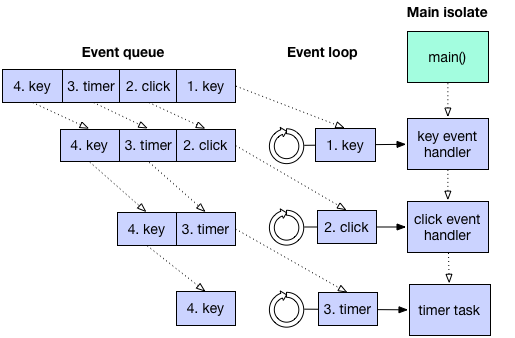
\includegraphics[scale=0.6]{event_loop}
		\caption[Event loop]{Illustrazione del funzionamento dell'\textit{event loop} \cite{event_loop}.}
		\label{figura:event_loop}
	\end{center}
\end{figure}

Un \textbf{event loop} \cite{isolate_event_loop_youtube} è una architettura asincrona che permette di inserire gli eventi generati in una coda e di gestirli uno alla volta estraendoli dalla coda ed eseguendo il rispettivo \textit{handler}. In particolare, viene preso l'evento più vecchio presente nella coda, viene eseguito il suo codice e torna ad estrarre un altro evento dalla coda, fino a quando la coda non è vuota. Questa architettura è stata pensata in quanto dal momento in cui viene avviata un'applicazione fino al momento in cui viene deallocata dalla memoria, l'applicazione non può prevedere quando dovranno essere elaborate delle operazioni di I/O, gestire il download di un file, gestire la UI ed altro ancora. Per di più, tutte queste operazioni devono essere gestite in un singolo thread che non si deve mai bloccare. Per questo motivo viene impiegato l'event loop. Ogni qualvolta si verifica un'interruzione, che può essere invocata ad esempio dall’interazione con l’utente o dalla risposta di una socket, l’event loop continua ad elaborare gli eventi fino a quando la coda non termina. In quel caso, il sistema attende la notifica di nuovi eventi. 

Tutte le API di alto livello e le funzionalità del linguaggio Dart per la programmazione asincrona, \verb|Future|, \verb|Stream|, \verb|async| e \verb|await| sono tutte basate sull'\textit{event loop}. In particolare, le API sono solo dei modi per notificare all'\textit{event loop} che è pronto del codice da eseguire. Gli \verb|Stream|, i \verb|Future| e \verb|async| e \verb|await| rappresentano le colonne portanti della programmazione asincrona in Dart.

\subsection{Future}
La problematica che può verificarsi durante l'esecuzione del codice nell'utilizzare un modello a singolo thread, è la possibilità di elaborare del \textit{codice bloccante}, il quale causerebbe il blocco il meccanismo dell'event loop. La programmazione asincrona viene utilizzata per risolvere questa problematica. Il tipo di dato \verb|Future<T>| è un’operazione asincrona che produce un risultato di tipo \verb|T| \cite{future_youtube}. Quando viene chiamato un metodo che restituisce un \verb|Future| succede che:
\begin{enumerate}
	\item Il metodo accoda le operazioni da eseguire;
	\item Al termine delle operazioni, il \verb|Future| viene completato con il risultato o con un
errore.
\end{enumerate}
Per poter utilizzare il risultato ottenuto da un metodo che restituisce un \verb|Future<T>|, vengono utilizzate delle \textbf{callback}.

Se il metodo non deve restituire alcun tipo di risultato allora il tipo di ritorno della funzione sarà \verb|Future<void>|.

\subsection{Async e await}
Nei linguaggi che supportano la programmazione asincrona, come ad esempio JavaScript, nella sintassi del linguaggio sono presenti le keyword \verb|async| e \verb|await|. \verb|async| viene utilizzato nella \textit{firma} di un metodo, per indicare che verrà restituito un \verb|Future|, o in un metodo in cui all'interno del suo corpo viene chiamato un metodo che restituisce un \verb|Future|. Mentre \verb|await| viene utilizzato per indicare di attendere che il \verb|Future| possa restituire il risultato. L'uso di \verb|await| permette di avere del codice non bloccante, permettendo all'event loop di proseguire e di non rimanere in attesa che il metodo termini. Quando le operazioni sono terminate, l'event loop riprenderà l'esecuzione dell'evento del \verb|Future| che ha prodotto il risultato.

\subsection{Stream}
Gli \verb|Stream| sono sequenze di eventi asincroni, che restituiscono un evento quando questo è terminato. Ad uno stato iniziale, lo \verb|Stream| è semplicemente un oggetto che contiene degli eventi al suo interno. Uno \verb|Stream| viene elaborato mediante l'uso di \verb|await| o mediante la callback \verb|listen()|. Quest'ultima, consente ad un \textit{Listener} di ascoltare lo \verb|Stream| e di estrarre gli eventi contenuti al suo interno.

In base alle esigenze, gli \verb|Stream| si suddividono in:
\begin{enumerate}
	\item \textbf{Single subscription stream}: gli eventi all'interno allo \verb|Stream| vengono restituiti tutti e in ordine. Questo flusso però può essere ascoltato da un solo \textit{Listener} un’unica volta. Il motivo è che un ulteriore ascolto può comportare la perdita degli eventi iniziali;
	\item \textbf{Broadcast stream}: questa modalità è destinata ai singoli messaggi che possono essere gestiti uno alla volta, come ad esempio gli eventi generati dal mouse. Più \textit{Listener} possono mettersi in ascolto sul medesimo \verb|Stream| di questa categoria e ci possono essere ascolti successivi senza che questi comportino la perdita di eventi.
\end{enumerate}

Ad uno \verb|Stream| possono essere collegai più \textit{Listener}. Quando è disponibile un nuovo evento, questo verrà notificato immediatamente a tutti gli ascoltatori collegati.

\subsection{dynamic}
Come è già stato spiegato precedentemente, Dart è un linguaggio fortemente tipizzato e supporta l'\textbf{inferenza} sui tipi. Quando però non viene dichiarato esplicitamente alcun tipo, viene implicitamente utilizzato il tipo \textbf{dynamic}. In Dart, ogni cosa è un oggetto che deriva dalla classe \verb|Object|. L’uso di \textit{dynamic} può significare che:
\begin{enumerate}
	\item È necessario rappresentare un tipo di dato non rientrante tra quelli consentiti;
	\item È necessario rappresentare un tipo di dato al di fuori dell'insieme dei tipi statici;
	\item Si dichiara esplicitamente il dinamismo per quel dato a tempo di esecuzione.
\end{enumerate}

Dal punto di vista dell'implementazione, questo significa che Dart non applica il controllo sul dato quando viene utilizzato \textit{dynamic}. Ad esempio, se si dichiara un dato di tipo \verb|A| e si prova a chiamare su quel dato un metodo non presente in \verb|A|, Dart avvisa dell'errore. Se inveve il tipo è stato dichiarato con \verb|dynamic|, è possibile chiamare qualsiasi metodo, anche se questo genererà un errore a tempo di esecuzione, in quanto Dart smette di applicare a tale dato il meccanismo di controllo statico.

\subsection{Gestore dei pacchetti}
\textbf{Pub} è uno strumento per la gestione dei pacchetti per Dart \cite{pub}. È una raccolta di plugin \textit{open source} che possono essere poi inclusi ed utilizzati nelle varie applicazioni. Sono presenti pacchetti sia per Flutter ma anche per Dart Web, Linux, macOS e Windows.

\section{Familiarità della sintassi}
La sintassi del linguaggio Dart è molto simile alla sintassi dei linguaggi Java, JavaScript e di altri linguaggi. A supporto di quanto appena affermato, si illustrano alcuni pezzi di codice scritti in diversi linguaggi che implementano il medesimo codice \cite{confronto_linguaggi}:
\begin{enumerate}
\item \textbf{Dart}


\lstset{numbers=left, % vogliamo numerare le righr
  numberstyle=\tiny, % i numeri sono piccoli
  basicstyle=\ttfamily, % usiamo il carattere dattilografico
  columns=fullflexible, % niente emulazioni di allineamento
  backgroundcolor=\color{lightgray}, % colore di sfondo
  language=Java, % linguaggio usato
  }
\begin{lstlisting}
class Segment {
	int links = 4;
	toString() => "I have $links links";
}
\end{lstlisting}

\item \textbf{Kotlin}
\begin{lstlisting}
class Segment {
	var links:  Int = 4
	override fun toString() => 
		"I have $links links"
}
\end{lstlisting}

\newpage

\item \textbf{Swift}
\begin{lstlisting}
class Segment: CustomStringConvertible {
	var links:  Int = 4
	public var description: String { return
		"I have \(links) links"
	}
}
\end{lstlisting}

\item \textbf{TypeScript}
\begin{lstlisting}
class Segment {
	links: number = 4
	public toString() = () : string => { return
		'I have ${this.links} links'
	}
}
\end{lstlisting}
\end{enumerate}

\section{Confronto con JavaScript}

\subsection{Introduzione a JavaScript}
JavaScript è un linguaggio di \textit{scripting} interpretato che permette di realizzare applicazioni sia \textit{lato client} che \textit{lato server}. È il linguaggio di scripting che viene maggiormente usato nel contesto del Web. JavaScript è un linguaggio \textit{prototype-based} ed \textit{event-driven}.

Contrariamente a quanto suggerisce il nome, JavaScript non ha alcuna correlazione con il linguaggio di programmazione \textit{Java}, se non per la sintassi. Il nome è stato scelto per ragioni di marketing piuttosto che per la vicinanza dei due linguaggi.

JavaScript non produce delle applicazioni completamente \textit{stand-alone} ma necessitano di essere eseguite in un determinato ambiente. Nel caso di applicazioni lato client, queste vengono eseguiti nel \textit{browser}. I programmi lato server, come ad esempio quelli realizzati in \textit{Node.js}, vengono eseguiti grazie ad uno specifico \textit{engine}. Sia Google Chrome che Node.js utilizzano lo stesso engine: il \textit{V8} sviluppato da Google. 

L’uso principale di JavaScript è in ambito Web per la realizzazione di potenti applicazioni Web dinamiche.

\subsection{Confronto}

\subsubsection{Class-based e prototype-based}
Come prima differenza possiamo notare che Dart è un linguaggio \textit{class-based} e non \textit{prototype-based} come \textbf{JavaScript}. Quest'ultimo è un linguaggio che si basa sugli \textit{oggetti} e non prevede l’utilizzo delle \textit{classi}. Le classi sono dei costrutti utilizzati come modelli per la creazione degli oggetti. Ogni modello può contenere degli attributi e dei metodi.
\textbf{Dart}, a differenza di JavaScript, essendo un linguaggio class-based, integra il concetto di \textit{interfaccia}, di classe e di oggetti che vengono istanziati a partire da esse.

\subsubsection{Curva di apprendimento}
Supponendo di conoscere i concetti di base della programmazione, l'apprendimento di \textbf{JavaScript} risulta essere semplice. C'è un'ampia letteratura online ed offline riguardo questo linguaggio e tutte le sue peculiarità.

Sulla base delle medesime considerazioni iniziali, la curva di apprendimento di \textbf{Dart} risulta essere leggermente più alta rispetto a quella di JavaScript. La causa è dovuta alla scarsa diffusione del linguaggio e alla poca letteratura che è stata prodotta a riguardo. La documentazione più prolissa è quella fornita da Google. Le similitudini a livello sintattico con JavaScript e Java aiutano molto l'apprendimento a quei sviluppatori che provengono appunto da esperienze con tali linguaggi.

\subsubsection{Semplicità d'uso del linguaggio}
\textbf{JavaScript} è nato nel 1995 ed è conosciuto da molti programmatori. È uno dei linguaggi più diffusi ed utilizzati nel mondo. È un linguaggio maturo, stabile ed è molto facile da utilizzare. Vi sono numerosi framework e librerie scritti in questo linguaggio.

\textbf{Dart} è un linguaggio relativamente recente per la maggior parte degli sviluppatori. Sebbene Google abbia fatto molti sforzi per documentare il linguaggio, è ancora difficile per gli sviluppatori trovare delle soluzioni a dei specifici problemi.

\subsubsection{Compilazione ed interpretazione}
\textbf{Dart} è un linguaggio compilato e questo permette di trovare la gran parte degli errori di programmazione a tempo di compilazione. Essendo inoltre \textit{type safe}, è più sicuro dal punto di vista della tipizzazione rispetto a JavaScript, rendendo più semplice il debugging delle applicazioni. \textbf{JavaScript} è un linguaggio \textit{debolmente tipizzato} ed interpretato, caratteristica strutturale che degrada le prestazioni dell'applicazione. Inoltre Dart, può essere compilato AOT o JIT in base alle esigenze e ai contesti.

\subsubsection{Web e mobile}
\textbf{JavaScript} è sicuramente il linguaggio che viene per la maggior parte utilizzato durante lo sviluppo di applicazioni mobili e Web grazie a diversi framework. JavaScript è alla base di molti framework che permettono di realizzare Web app, PWA, applicazioni ibride e cross-platform.

Analogamente a JavaScript, \textbf{Dart} può essere utilizzato sia per lo sviluppo mobile che Web. Tuttavia il successo del linguaggio è dovuta al framework \textit{Flutter}. Quindi, in questo periodo, Dart viene identificato più come un linguaggio adatto per costruire applicazioni multipiattaforma che per sviluppare applicazioni per il Web.